\section{Problem statement}

A bi-axial shear test of a homogenous material block of $\SI{1}{\metre} \times
    \SI{1}{\metre} \times \SI{1}{\metre}$ should be modeled to test the limit load
resulting from the Mohr-Coulomb failure criterion. The test setup is shown in
\autoref{bi-axial-shear-mohr-coulomb::fig:setup}. At xmin, ymin, ymax, and zmin
the block is fixed perpendicular to the face. The face xmax is loaded with a
constant (normal) pressure of $\sigma'_2 =
    \qty{1}{\kilo\newton\per\square\metre}$. The (normal) pressure $\sigma'_1$ at
zmax ramps up till no convergence can be found anymore. Material parameters are
givin in \autoref{bi-axial-shear-mohr-coulomb:material-parameters}.

\begin{table}[htbp]
    \centering
    \caption{Material parameters}
    \label{bi-axial-shear-mohr-coulomb:material-parameters}
    \begin{tabularx}{\textwidth}{XYY}

        \hline

        Property                        & Physical unit                                         & Value       \\

        \hline

        Youngs modulus $E$              & \si[per-mode = symbol]{\kilo\newton\per\square\metre} &
        \SI{1000}{}                                                                                           \\

        Poisson's ratio $\nu$           & -                                                     & \SI{0.25}{} \\

        Angle of inner friction $\phi'$ & \si[per-mode = symbol]{\degree}                       & \SI{30}{}
        \\

        Cohesion $c'$                   & \si[per-mode = symbol]{\kilo\newton\per\square\metre} & 1           \\

        \hline
    \end{tabularx}
\end{table}

\begin{figure}[htbp]
    \centering
    \begin{tikzpicture}

        % this image has been generated using Blender writing a SVG
        % using the "Freestyle SVG Exporter". The SVG is minimized
        % using third-party tools and finally converted to PDF using
        % Inkscape.
        \node[inner sep=0pt] (ch-stresses) at (0,0) {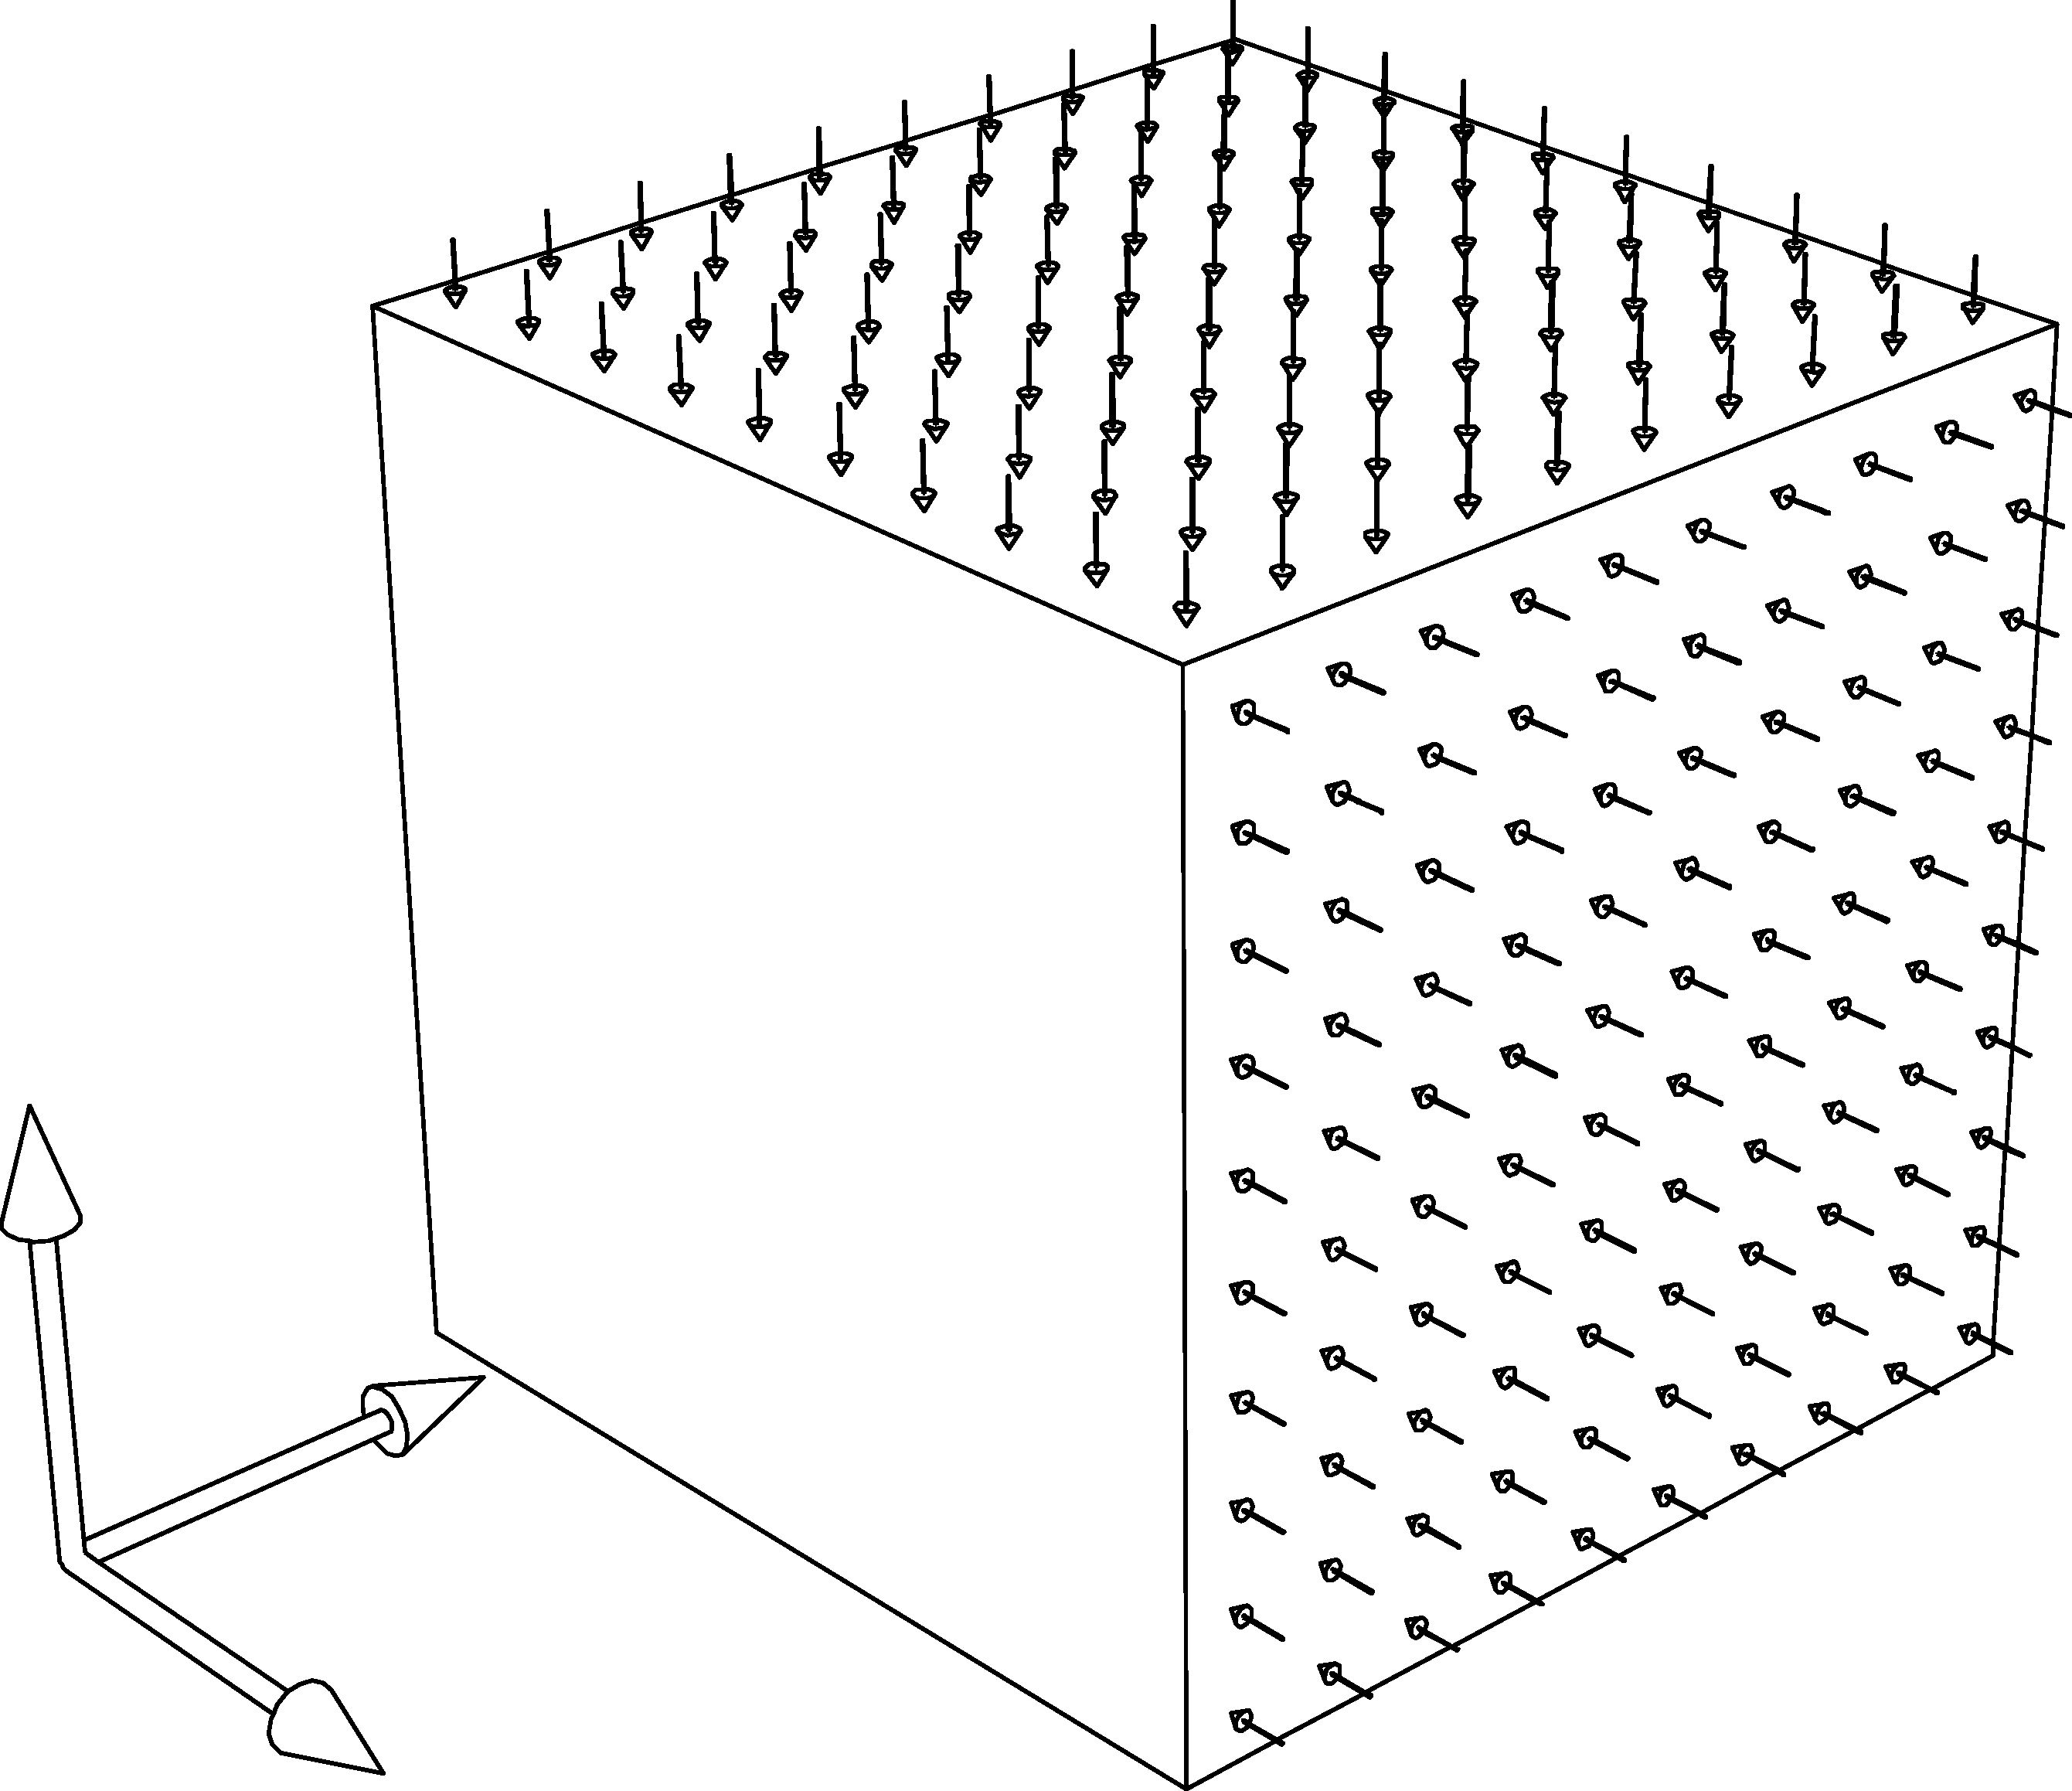
\includegraphics[width=0.4\linewidth]{\currfiledir/bi-axial-shear.blend.svg.pdf}};

        \node[] at (-3.0,-2.9) {x};
        \node[] at (-2.5,-1.5) {y};
        \node[] at (-3.0,-1.0) {z};

        \node[draw,circle,fill=white,minimum size=.5cm,inner sep=0pt, text width=1.5cm, align=center] (xmin_text) at (-4.0,+2.7) {xmin: $u_x \equiv 0$};
        \node (xmin) at (-2.1,+1.2) {};
        \path[->] (xmin_text) edge [out=0, in=180] (xmin);

        \node[draw,circle,fill=white,minimum size=.5cm,inner sep=0pt, text width=2.0cm, align=center] (xmax_text) at (+4.5,-2.5) {xmax: \\ $\sigma'_2 \equiv \qty[per-mode = fraction]{1}{\kilo\newton\per\square\metre} $};
        \node (xmax) at (+2.2,-1.4) {};
        \path[->] (xmax_text) edge [out=180, in=0] (xmax);

        \node[draw,circle,fill=white,minimum size=.5cm,inner sep=0pt, text width=1.5cm, align=center] (ymin_text) at (-3.8,+0.5) {ymin: $u_y \equiv 0$};
        \node (ymin) at (-0.8,-0.7) {};
        \path[->] (ymin_text) edge [out=0, in=180] (ymin);

        \node[draw,circle,fill=white,minimum size=.5cm,inner sep=0pt, text width=1.5cm, align=center] (ymax_text) at (+4.8,+1.7) {ymax: $u_y \equiv 0$};
        \node (ymax) at (+3.3,+0.0) {};
        \path[->] (ymax_text) edge [out=270, in=20] (ymax);

        \node[draw,circle,fill=white,minimum size=.5cm,inner sep=0pt, text width=1.5cm, align=center] (zmin_text) at (-1.2,-3.5) {zmin: $u_z \equiv 0$};
        \node (zmin) at (+0.2,-2.8) {};
        \path[->] (zmin_text) edge [out=0, in=270] (zmin);

        \node[draw,circle,fill=white,minimum size=.5cm,inner sep=0pt, text width=1.2cm, align=center] (zmax_text) at (+2.4,+3.2) {zmax: $\sigma'_1 = ?$};
        \node (zmax) at (+0.4,+1.7) {};
        \path[->] (zmax_text) edge [out=180, in=90] (zmax);

    \end{tikzpicture}
    \caption{Setup of the bi-axial shear test}
    \label{bi-axial-shear-mohr-coulomb::fig:setup}
\end{figure}

\section{Analytical solution}

From the yield function of the Mohr-Coulomb failure criterion shown in
\autoref{eqn:Mohr-Coulomb-failure-criterion} the limit load of the bi-axial
test can be derived as given in \autoref{eqn:bi-axial-test-limit-load}.

\begin{equation}
    \label{eqn:Mohr-Coulomb-failure-criterion}
    f = \frac{\abs{\sigma'_1 - \sigma'_2}}{2} + \frac{\sigma'_1 + \sigma'_2}{2} \cdot \sin{\phi'} - c' \cdot \cos{\phi'} = 0
\end{equation}

\begin{equation}
    \label{eqn:bi-axial-test-limit-load}
    \sigma'_1 = \sigma'_2 \cdot \frac{1 + \sin{\phi'}}{1 - \sin{\phi'}} - 2c' \cdot \frac{\cos{\phi'}}{1 - \sin{\phi'}}
    \approx \qty{-6.464}{\kilo\newton\per\square\metre}
\end{equation}

\section{Moose}

In the corresponding Moose model of this quasi-static problem a discretisation
of \qty{5184}{} TET10 elements and a transient executioner is used. The
linear-elastic material behaviour is modelled with a materials block of type of
\codeword{ComputeIsotropicElasticityTensor}. The ideal-plastic behaviour is
introduced with a materials block of type
\codeword{CappedMohrCoulombStressUpdate}. To avoid the cap of this materials
block to influence the system response, a very high tensile and compressive
strength is used.

The load $\sigma'_1$ ramps up linearly with time so that at $t =
    \qty{6.464}{\second}$ the load is $\sigma'_1 =
    \qty{-6.464}{\kilo\newton\per\square\metre}$. Due to the ideal-plastic nature
of the material behaviour, Moose will attempt to calculate time steps and
iteratively reduce the time step if convergence is not achieved. Eventually the
last converged time step should be at $t \approx \qty{6.464}{\second}$.

This model was calculated using the ‘PJFNK’ solver. The time step is initially
chosen to be \qty{0.25}{\second} and the minimum time step is limited to
\qty{0.001}{\second}. Due to the automatic cut-back of the time steps close to
failure, the last converged time step is at $t=\qty{6.43945}{\second}$. The
Moose input file for this model is attached to this document by the name of
‘bi-axial-shear.i’.

\fileattachment{\currfiledir/bi-axial-shear.i}{bi-axial-shear.i}

\section{Plaxis 3D}

The mesh used for Plaxis3D consists of 5130 TET10 elements.